\documentclass[10pt,a4paper]{book}
\usepackage{graphicx}
 % Requires \usepackage{graphicx}

\begin{document}

\small

\begin{flushleft}
  \textsf{\textbf{324 $|$ Introduction to Automata Theory, Formal Languages and Computation}}
\end{flushleft}

ii) A → (00)*00 S → (01)*S/1(00)*00

\quad

\qquad\qquad\qquad\qquad\qquad S → (01)*1(00)*00

\quad

\quad The regular expression is (01)*1(00)*00.

iii) Reversing the regular expression, we get 00(00)*1(01)*.

iv) The fi nite automata constructed from the expression in step III is

\begin{figure}[h]
  \centering
  % Requires \usepackage{graphicx}
  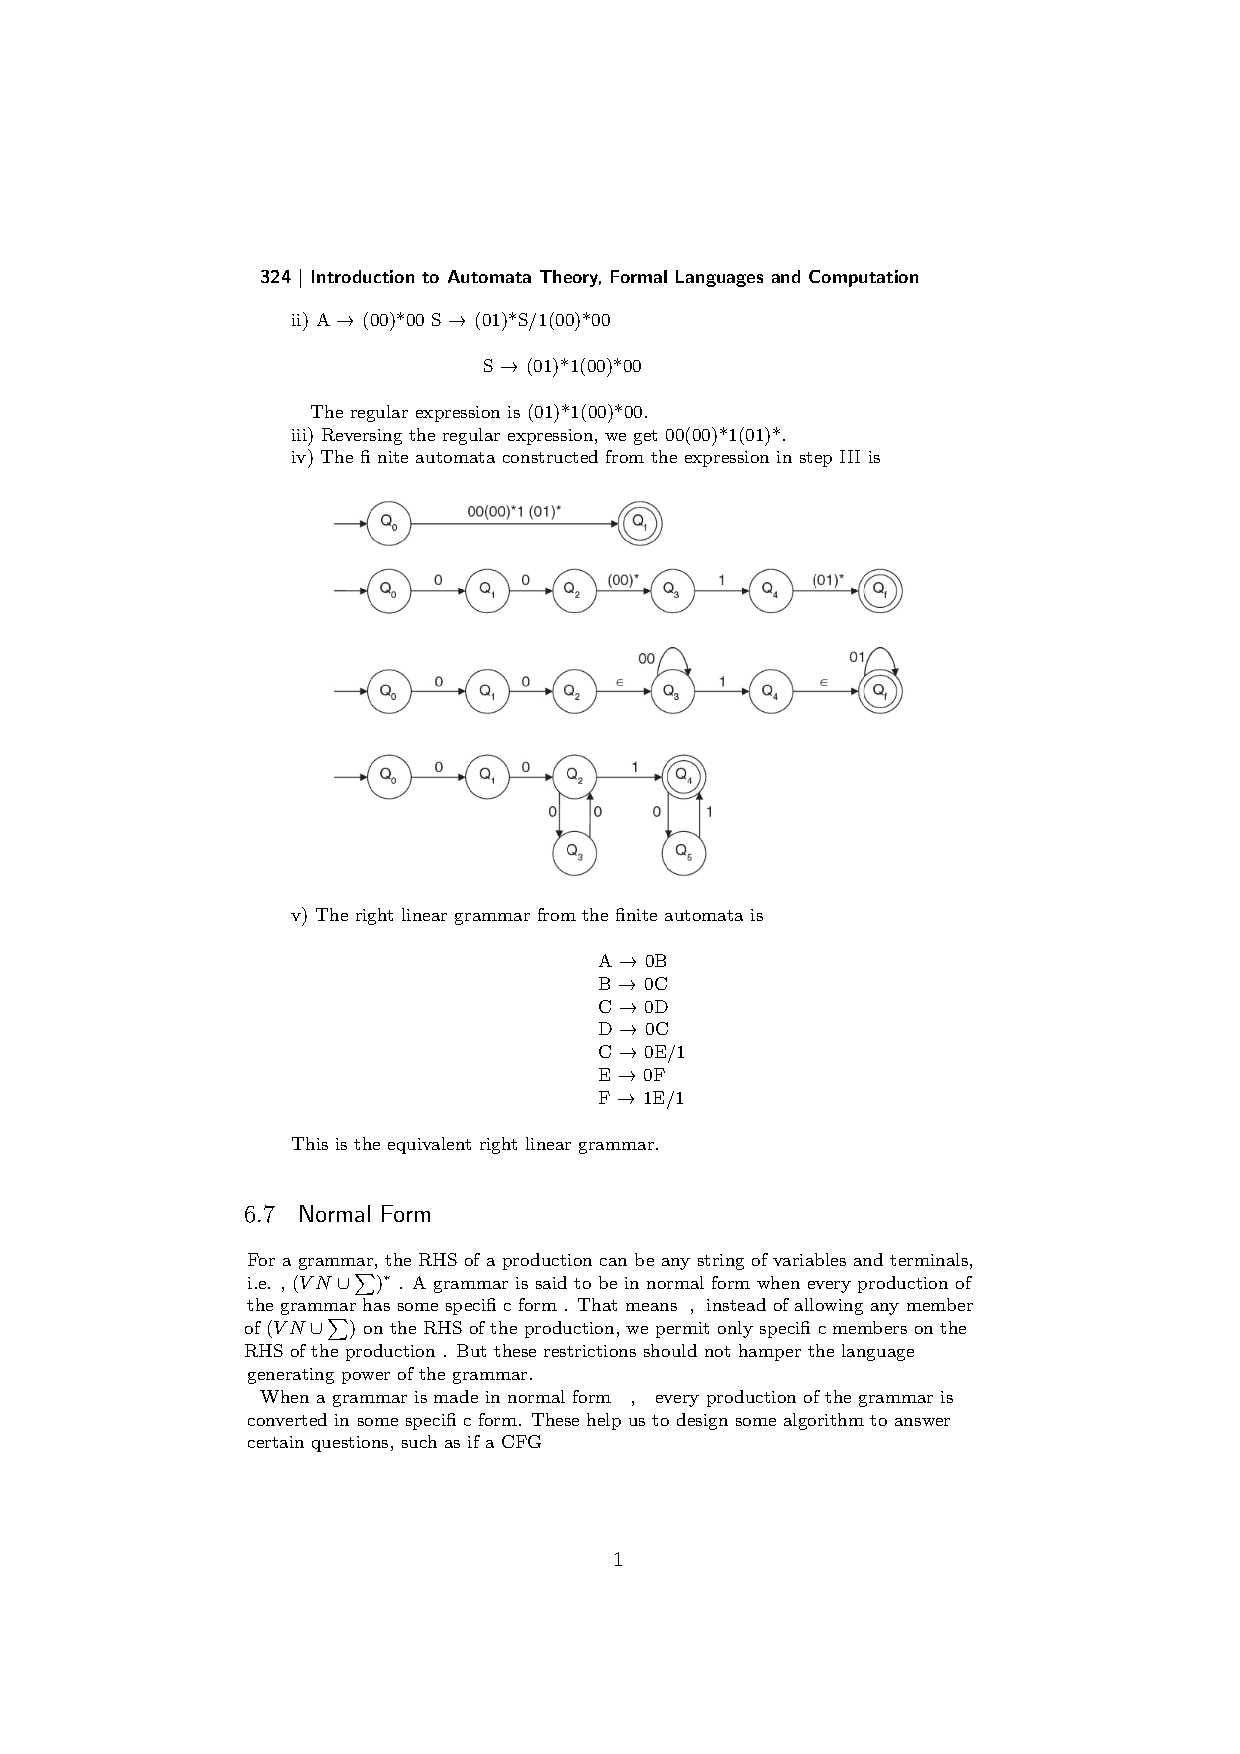
\includegraphics[width=10cm]{324}\\
\end{figure}

v) The right linear grammar from the finite automata is

\quad

\qquad\qquad\qquad\qquad\qquad\qquad\qquad\qquad A → 0B

\qquad\qquad\qquad\qquad\qquad\qquad\qquad\qquad B → 0C

\qquad\qquad\qquad\qquad\qquad\qquad\qquad\qquad C → 0D

\qquad\qquad\qquad\qquad\qquad\qquad\qquad\qquad D → 0C

\qquad\qquad\qquad\qquad\qquad\qquad\qquad\qquad C → 0E/1

\qquad\qquad\qquad\qquad\qquad\qquad\qquad\qquad E → 0F

\qquad\qquad\qquad\qquad\qquad\qquad\qquad\qquad F → 1E/1

\quad

This is the equivalent right linear grammar.

\qquad

\begin{flushleft}
  \!\!\!\!\!\large 6.7 \; \textsf{Normal Form}
\end{flushleft}
\begin{flushleft}

\!\!\!\!For a grammar, the RHS of a production can be any string of variables and terminals,

\!\!\!\!i.e. , $(VN \cup \sum)^{*}$ . A grammar is said to be in normal form when every production of
 
\!\!\!\!the grammar has some specifi c form .
That means\; ,\; instead of allowing any member
 
\!\!\!\!\!of $(VN \cup \sum)$ on the RHS of the production, we permit only
specifi c members on the
 
\!\!\!\!\!RHS of the production . But these restrictions should not hamper the language

\!\!\!\!generating power of the grammar.

When a grammar is made in normal form\quad,\quad every production of the grammar is

\!\!\!\!converted in some specifi c form. These help us to design some algorithm to answer
 
\!\!\!\!certain questions, such as if a CFG
\end{flushleft}







\end{document}
